% Document

\section{Background}\label{sec:Background}

    \subsection{Agent-Based Modeling}\label{subsec:abm}
        The agent-based modeling methodology has matured and its applications expanded
        in recent years [Collins, 2015] and software tools for agent-based modeling
        are available [Wilensky, 2015].
        Agent-based modeling models systems that are composed of multiple distinct agents
        that interact with each other and their environment.
        Agents sense the environment, adapt their behaviors to the environment,
        and may alter their environment.
        According to [Macal, 2010], agents are modular and autonomous entities that have a
        state that varies with time and that interact with other agents in manners that
        affect behavior.
        Agents' behaviors may result in changes to the environment which, in turn, may
        influence the later behaviors of other agents.
        Simulations using agent-based models may reveal unanticipated relationships
        and configurations.
        Modeling the agents as independent units facilitates arrangements that emerge
        from the autonomous decisions and behaviors of those agents.

    \subsection{Population Dynamics}\label{subsec:population-dynamics}
        When modeling population dynamics, differential equations can be used to
        approximate the behavior of species with large populations.
        Using one or more equations, we can produce an analytical solution to the
        population model that is easy to compute and will provide good accuracy
        if the population is sufficiently large.
        Using an analytical solution, however, introduces a few obvious issues.
        First, to use a system of differential equations, real numbers must be used.
        It becomes problematic to have fractional population members.
        These analytic solutions also disregard any biological constraints,
        such as requiring two of a species to reproduce.
        If these issues can be tolerated, it becomes very simple to model a population.
        To model a single population without any constraining factors,
        we can use the Malthusian growth model.
        Using a constant growth and death rate, we can use the following equation
        to predict the population at time $t$ using an initial population $P_{0}$
        and a growth rate of $r$.
        \begin{equation}\label{eq:malthusian}
            P(t) = P_{0} \cdot e^{rt}
        \end{equation}
        In any realistic environment, ~\ref{eq:malthusian} will not work, as the population
        will continue to grow exponentially with time.
        To address the issue of limited resources we can use a logistic growth model.
        Here we will introduce a saturation point that the model will eventually converge.
        Here we choose $a \gg b > 0$, this causes the rate of change of $p$ to become $0$
        when $p = a/b$ or when $p = 0$. [Bungartz 2014]
        \begin{equation}\label{eq:logistic}
            \displaystyle p(t) =
            \frac{a \cdot p_0}{b \cdot p_0 + (a - b \cdot p_0) \cdot e^{-at}}
        \end{equation}
        Systems of differential equations can also be used to model populations of two
        or more species.
        With populations of two species, there can be various relationships.
        The species can either be in competition for the same resource,
        exist as a predator-prey relationship, or non-interactive.
        Non-interacting species are typically not interesting since they can be
        modeled independently.
        The other two relationships will experience different behaviors.
        We will focus on the predator-prey relationship since it is the focus of
        our experiment.
        To model two species populations, we can choose values for
        $a_1$, $a_2$, $b_1$, $b_2$, $c_1$, and $c_2$ such that:
        \begin{equation}\label{eq:inequality}
            \displaystyle \frac{b_1}{c_2} > \frac{a_1}{a_2} > \frac{c_1}{b_2}
        \end{equation}
        For these values, the population of the predator species $\overline{p}$ and
        prey species $\overline{q}$ will converge to the following stable values. [Bungartz 2014]
        \begin{equation}\label{eq:convergence}
            \displaystyle \overline{p} = \frac{a_1 b_2 - c_1 a_2}{b_1 b_2 - c_1 c_2}, \,\,
                          \overline{q} = \frac{b_1 a_2 - a_1 c_2}{b_1 b_2 - c_1 c_2}
        \end{equation}
        When modeling predator-prey relationships, we can choose
        $b_1 = b_2 = 0$ corresponding to no restriction to the population
        of one's own species.
        This will cause an oscillating pattern to occur.
        As the prey's species becomes large, the predator's population will also grow.
        This will then cause the prey's species to quickly die off,
        followed by the predator's, as resources become constrained.

    \begin{figure}[H]
        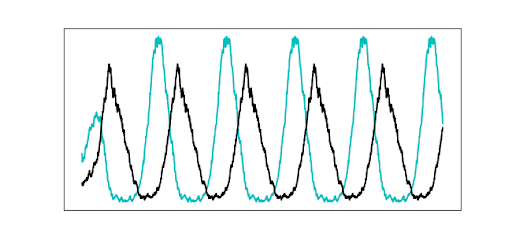
\includegraphics[width=\linewidth]{./figures/population_dynamics}
        \caption{\textit{
           Model of a predator-prey relationship demonstrating the oscillating behavior.
           As the prey species (blue) increases, it triggers an increase in the
           predator (black) species.
           This will cause the prey to die off, followed by the predator.
           This cycle repeats indefinitely in the continuous case.}}
        \label{fig:population_dynamics}
    \end{figure}

        In ~\ref{fig:population_dynamics} the population will continue to oscillate forever.
        As noted earlier, however, this is only true in the continuous case.
        When used to model a discrete population, the predator-prey case is often
        unstable with only two species.

        Modeling discrete populations becomes significantly more difficult as birth
        and death rates produce integer changes in the population and must be modeled
        as random events.
        Rather than determining the value of the population directly, we will model
        the probability of the population being of specific size.

        If we assume the growth and death rates are constant we can derive the
        following equation:
        \begin{equation}\label{eq:discrete_population}
            \pi_x(t + \delta t) =
            \pi_x(t) - \gamma x \delta \pi_x(t) + \gamma(x - 1)\delta t \pi_{x - 1}(t)
        \end{equation}
        with $\gamma$ representing the combination of birth and death rates,
        and $\delta t$ representing a tiny step in time that approaches $0$.
        With this we can use an infinite series of equations to model a
        discrete population.
        By choosing a small fixed value of $\delta t$ we can then approximate
        the population at time $t$ numerically. [Bungartz 2014]

        Modeling discrete populations, especially ones with multiple species,
        becomes extremely difficult.
        In these cases it is often helpful to use an agent-based simulation
        to find a possible solution to the desired problem.

    \subsection{NetLogo and the Wolf Sheep Predation model}\label{subsec:netlogo-wsp}
        NetLogo's Wolf Sheep Predation model is a highly abstracted simulation of a
        predator-prey ecosystem consisting only of wolves, sheep, and grass.
        The populations of these three species are interrelated, as wolves consume sheep,
        sheep consume grass, and grass is depleted and restored over time.
        In this model, shown in ~\ref{fig:NetLogo WSP} animals have a chance to reproduce asexually each time-step based
        on the animal's reproductive rate.
        When an animal reproduces, its energy is split between the parent and the child.
        When an animal's energy is depleted, it perishes and is removed from the simulation.

    \begin{figure}[H]
        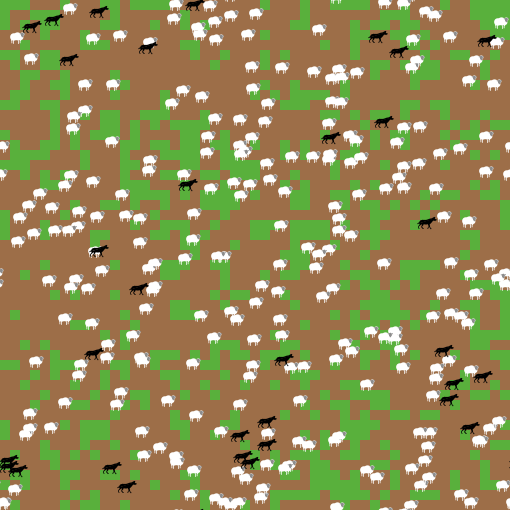
\includegraphics[width=\linewidth]{./figures/netlogo_wsg}
        \caption{\textit{
           A screenshot of NetLogo's Wolf Sheep Predation model [Wilensky 1997].}}
        \label{fig:NetLogo WSP}
    \end{figure}

        The simulation terrain is a square grid of green or brown squares,
        each of which represents a patch of grass in one of two states:
        an incomplete growth cycle, or a completed growth cycle.
        Sheep can only eat a patch of grass if it is in the green state.
        After being consumed, the patch becomes brown, and then a certain amount
        of time passes before it finishes its growth cycle and becomes green again.
        Wolves and sheep follow random paths on the grid and do not seek out food or
        run from predators.
        When a wolf encounters a sheep, it will eat that sheep and gain some energy.
        When a sheep eats grass, the sheep gains some energy, and the grass restarts
        its growth cycle.
        Each turn, all wolves and sheep lose one unit of energy.